%
%
%
%
%
\section{Great Britain Transportation Networks Results: Air and Coach Travel} 
\label{app:air_and_coach}

For completeness, we include figures and persistence diagrams for the Great Britain transportation data not included in Sec.~\ref{ssec:GB_results}. 

\subsection{Coach Travel Network Analysis}
Figure~\ref{fig:GB_coach_all} shows the full network for the coach data, and the 0- and 1-dimensional zigzag diagrams in the top row. 
The standard statistics for temporal graphs are shown in the bottom row. 
See Sec.~\ref{ssec:coach} for a full discussion of the coach data. 
%


%
\subsection{Air Travel Network Analysis}
Figures~\ref{fig:GB_air_all} shows the zigzag diagrams and standard measures for the air travel data. 
Like rail and coach, the air travel network clearly has regular daily structure as seen in both diagrams. 
Interestingly, here we have a daily persistence point in 0-dimensions with splits in the middle, meaning that the air network does not retain any connected regions overnight. 
This, again, is not surprising as there is more tendency for airports to have absolutely no flights overnight as opposed to late-night bus systems. 
The lack of high persistence points in $H_1$ suggests that there are not even many small loops in the network at any given time, which might be caused by having considerably fewer edges in this network than the others. 


\begin{figure}
     \centering
     %
     
     \begin{minipage}{0.3\textwidth}
         \centering
         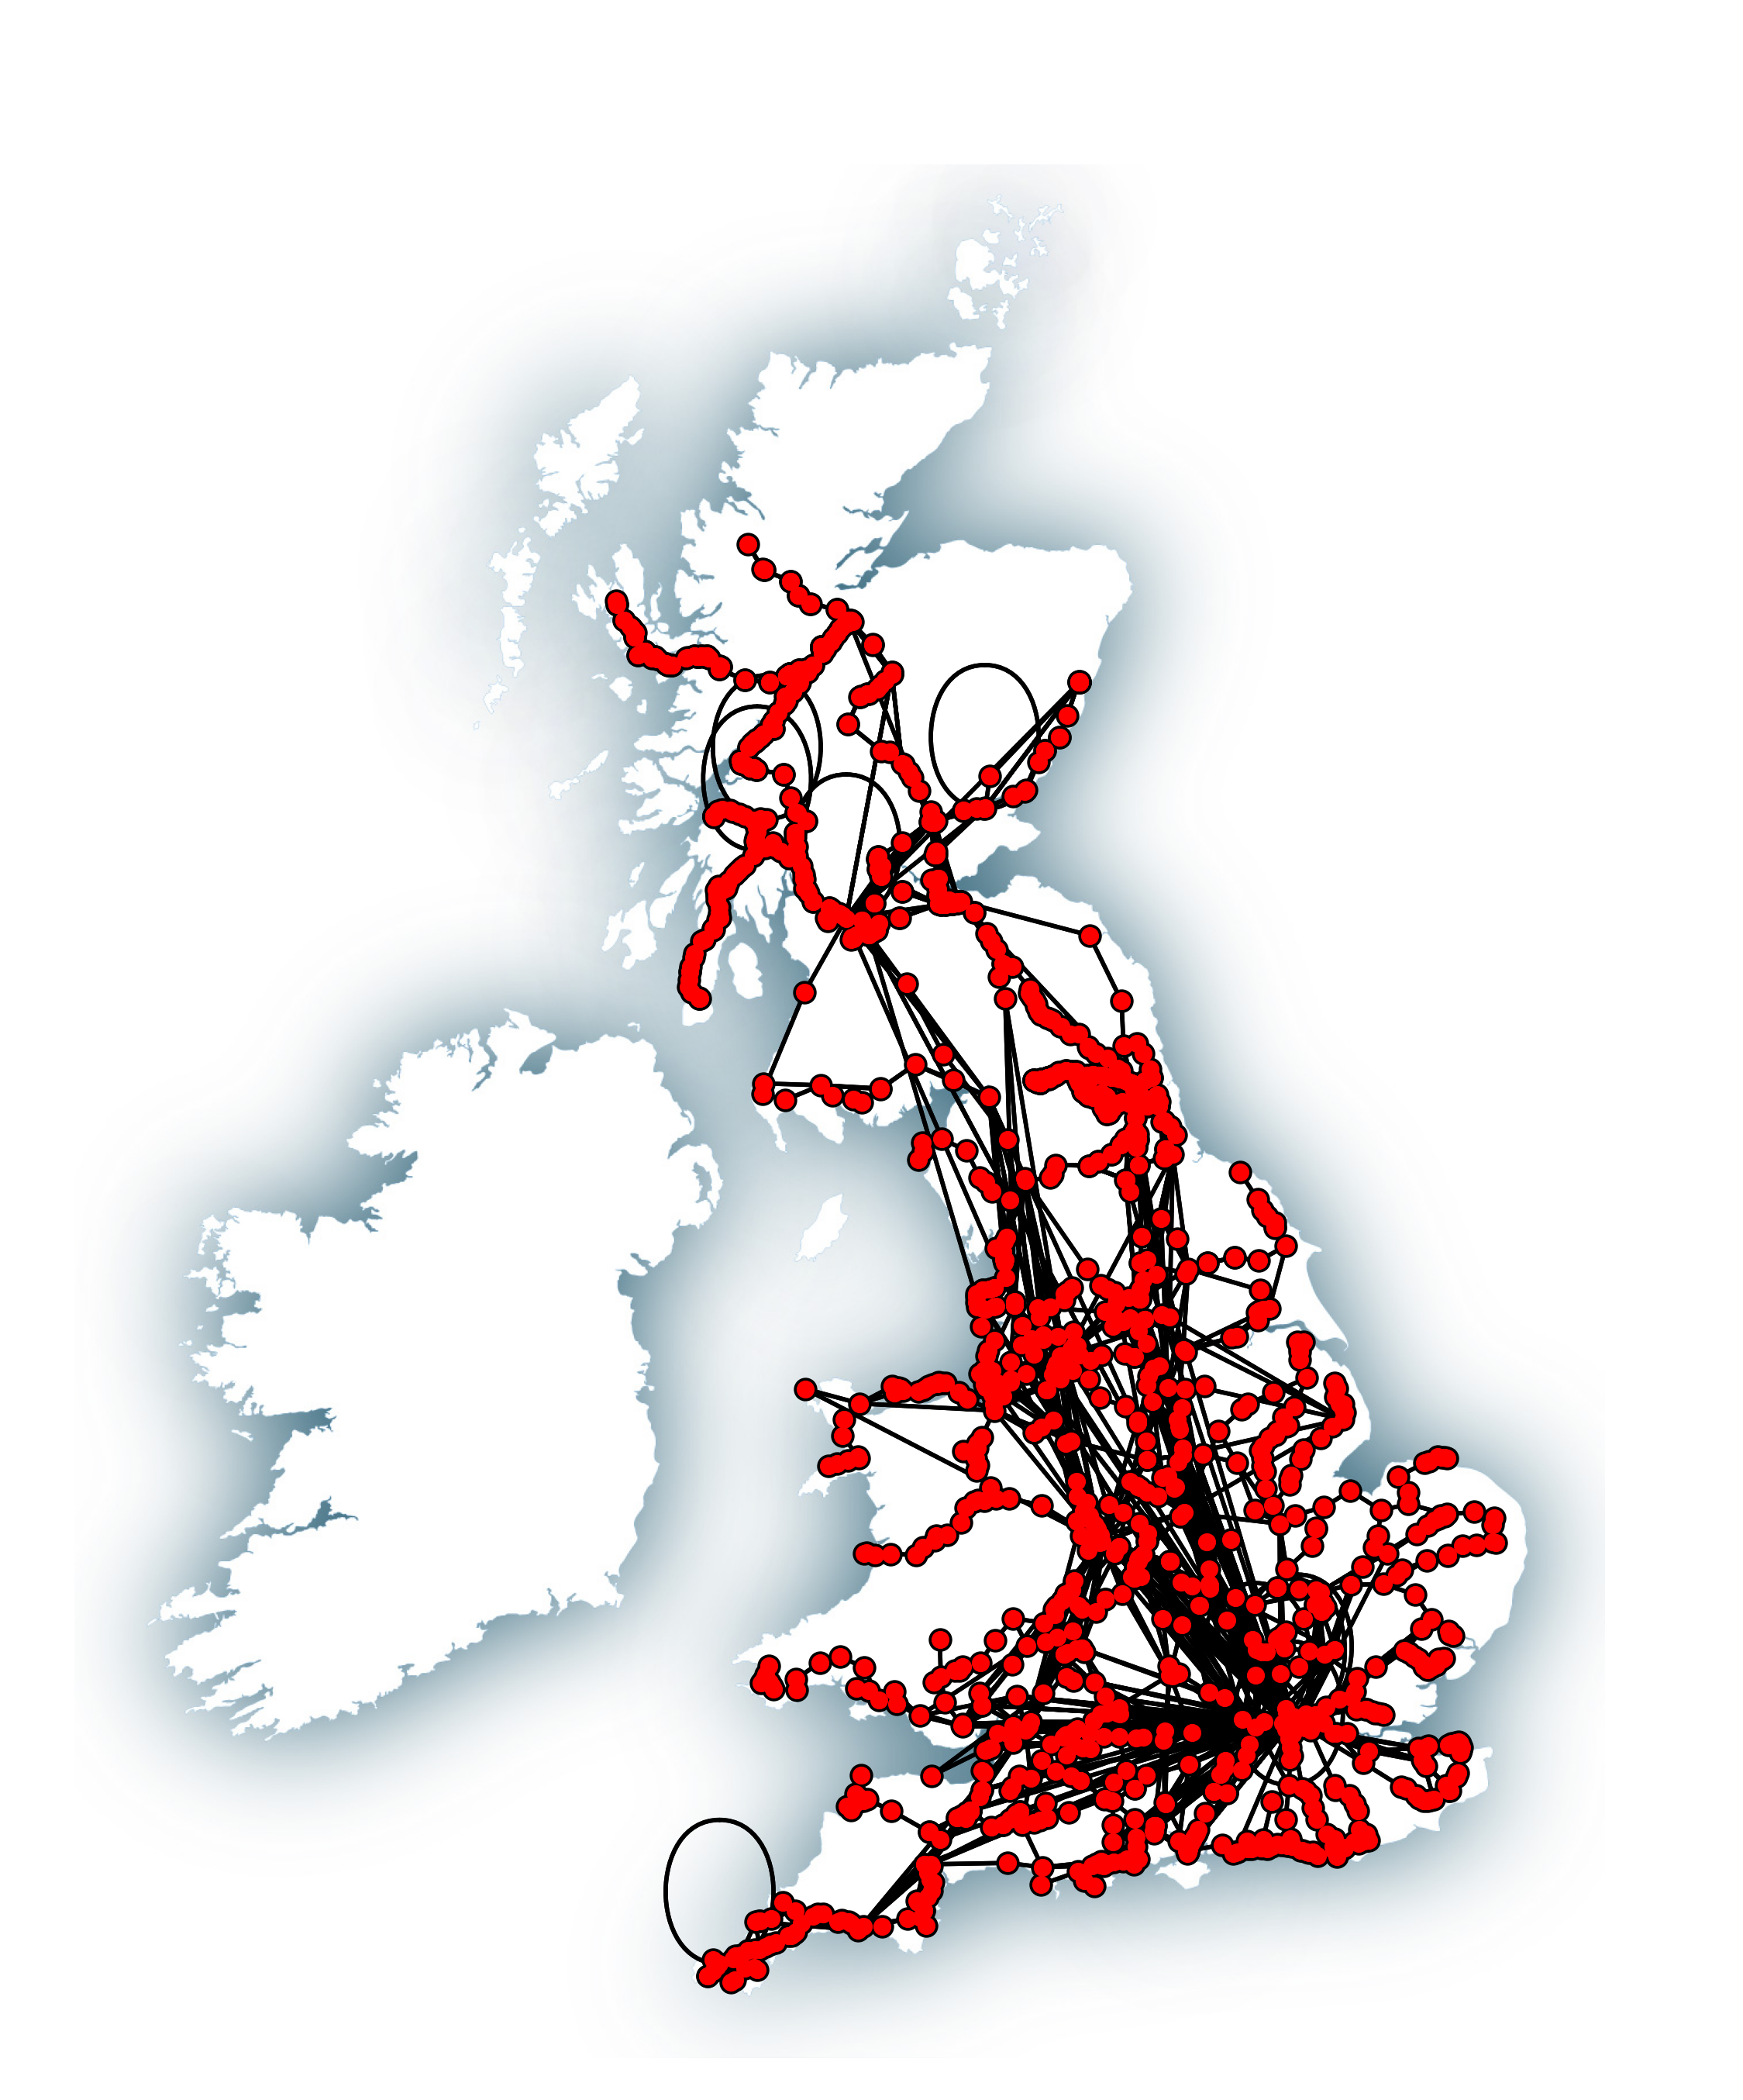
\includegraphics[width=\textwidth]{Figures/GB_coach} \\
         (a) Full coach Travel Network.
         %
         %
     \end{minipage}
     \hfill
     \begin{minipage}{0.3\textwidth}
         \centering
         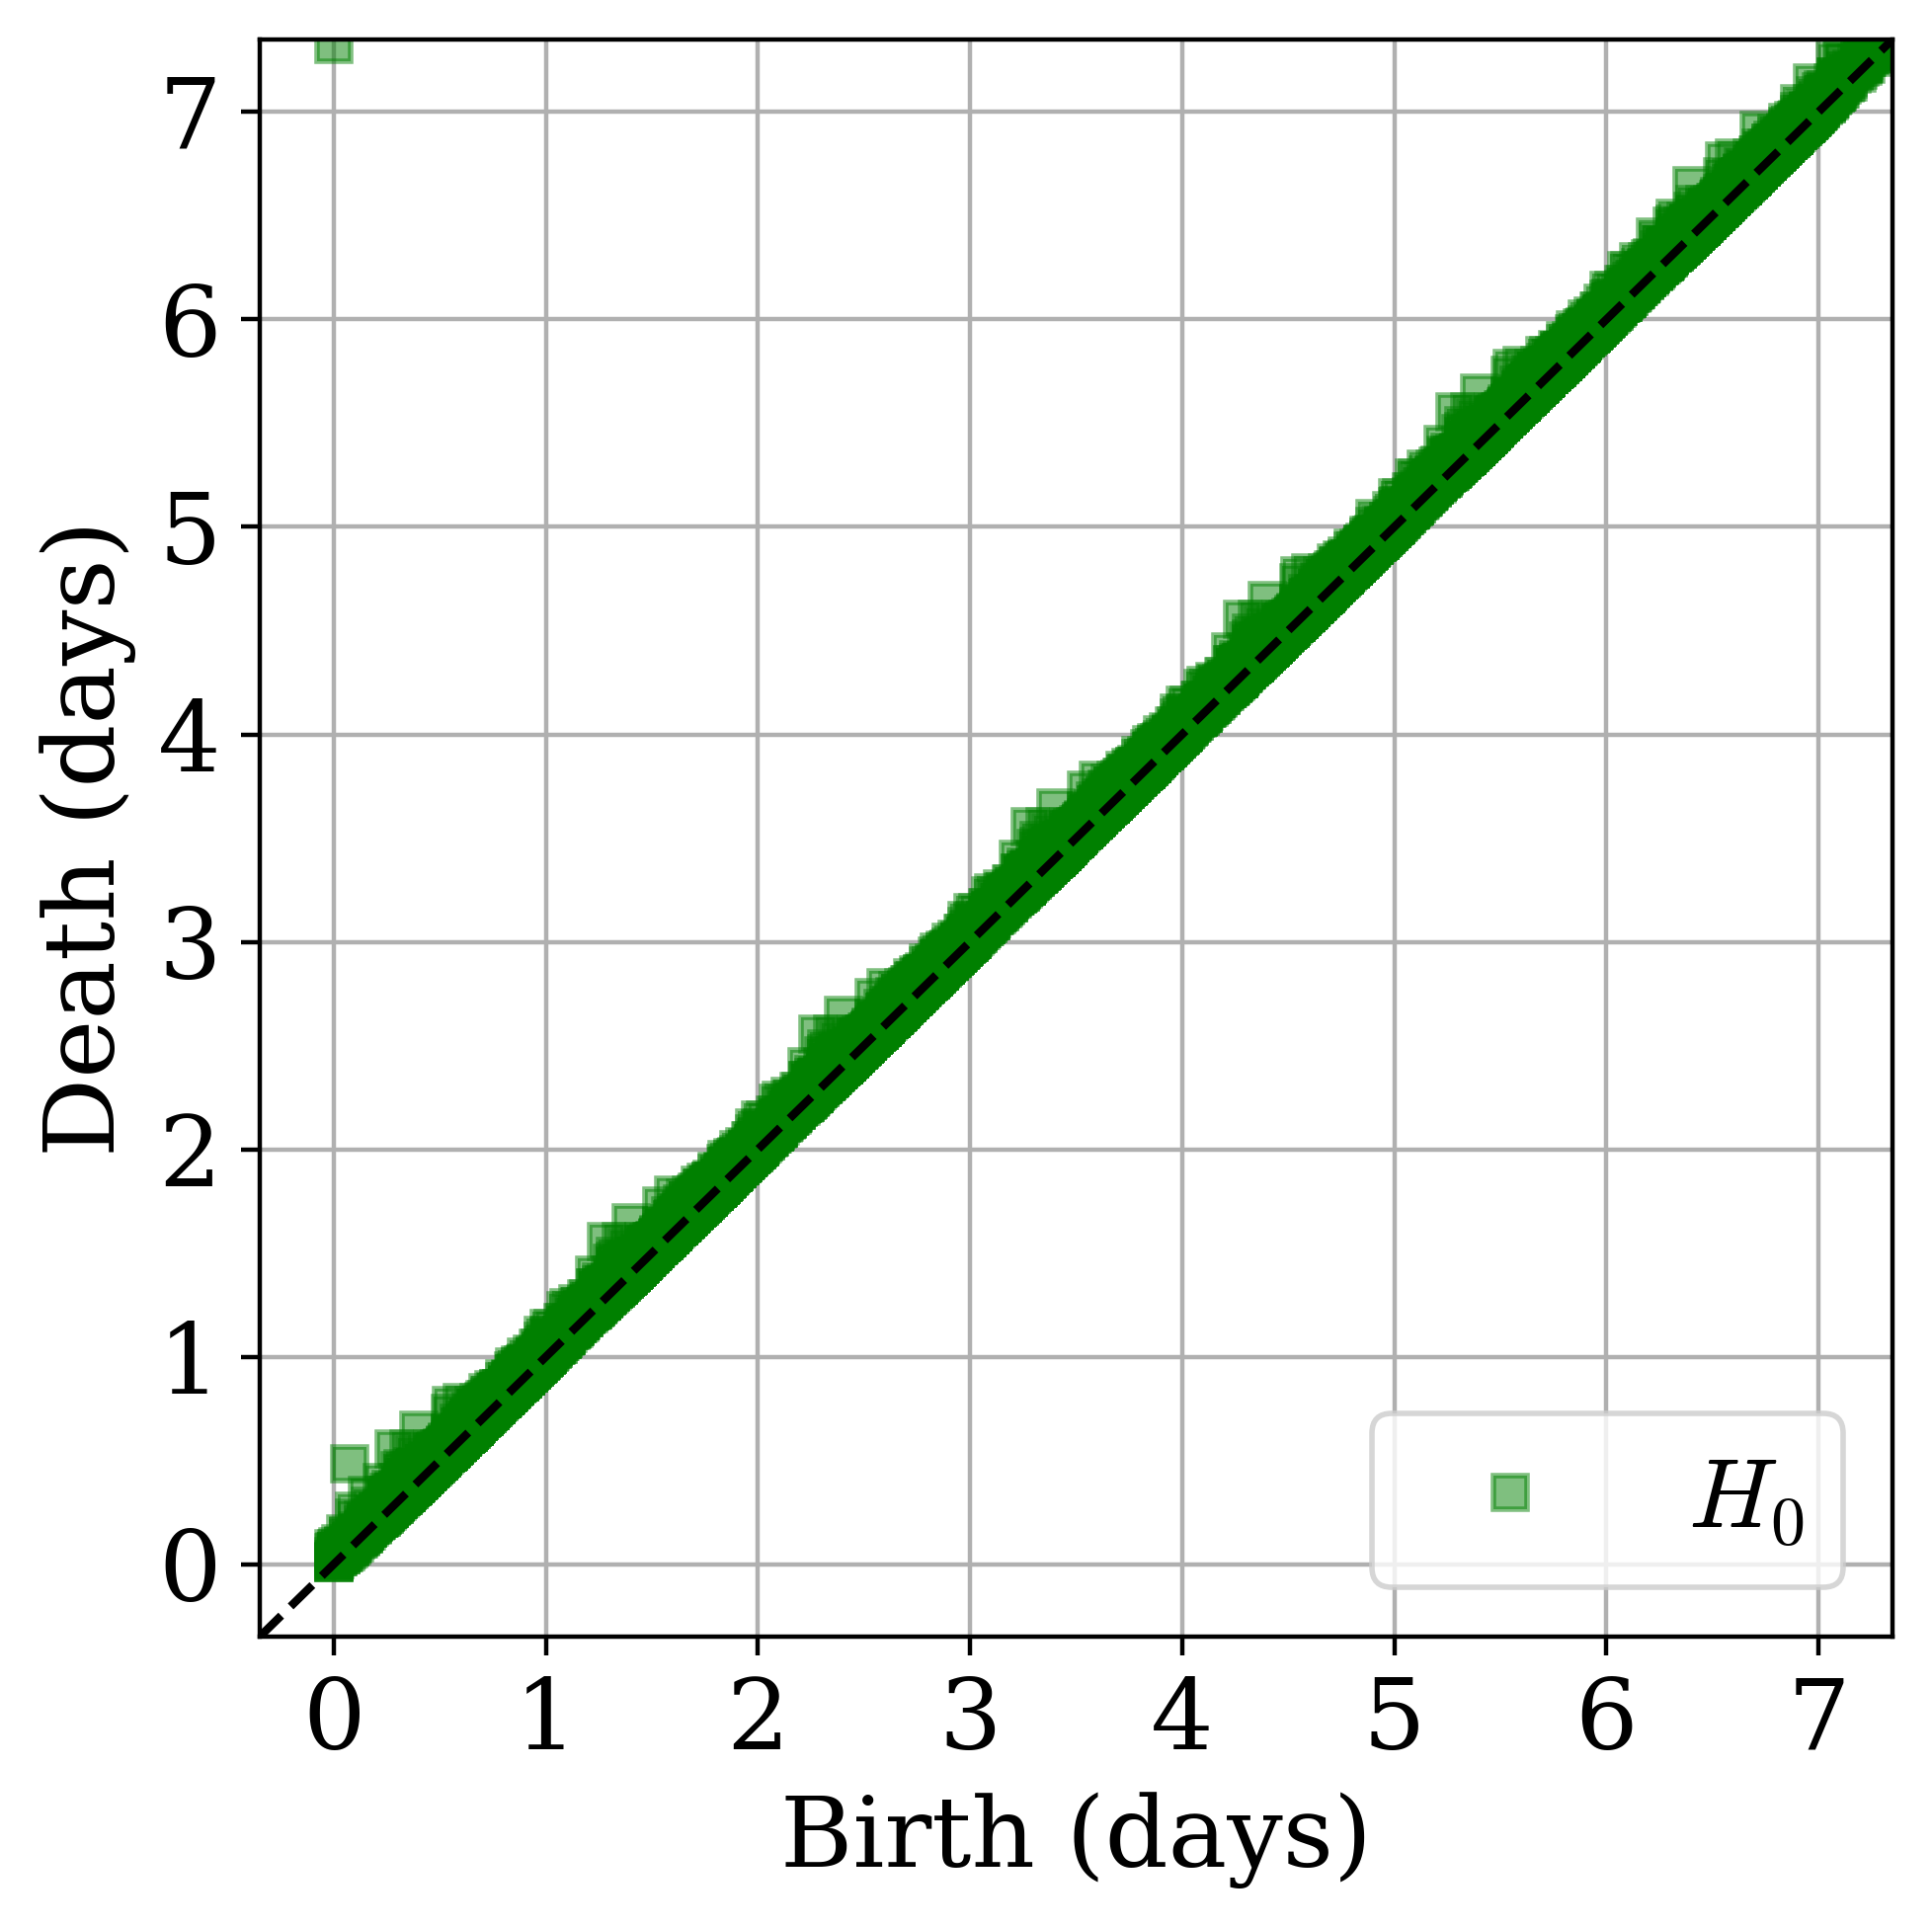
\includegraphics[width=\textwidth]{Figures/GB_coach_PD0} \\
         (b) Zero-dimensional zigzag persistence.
         %
         %
     \end{minipage}
     \hfill
     \begin{minipage}{0.3\textwidth}
         \centering
         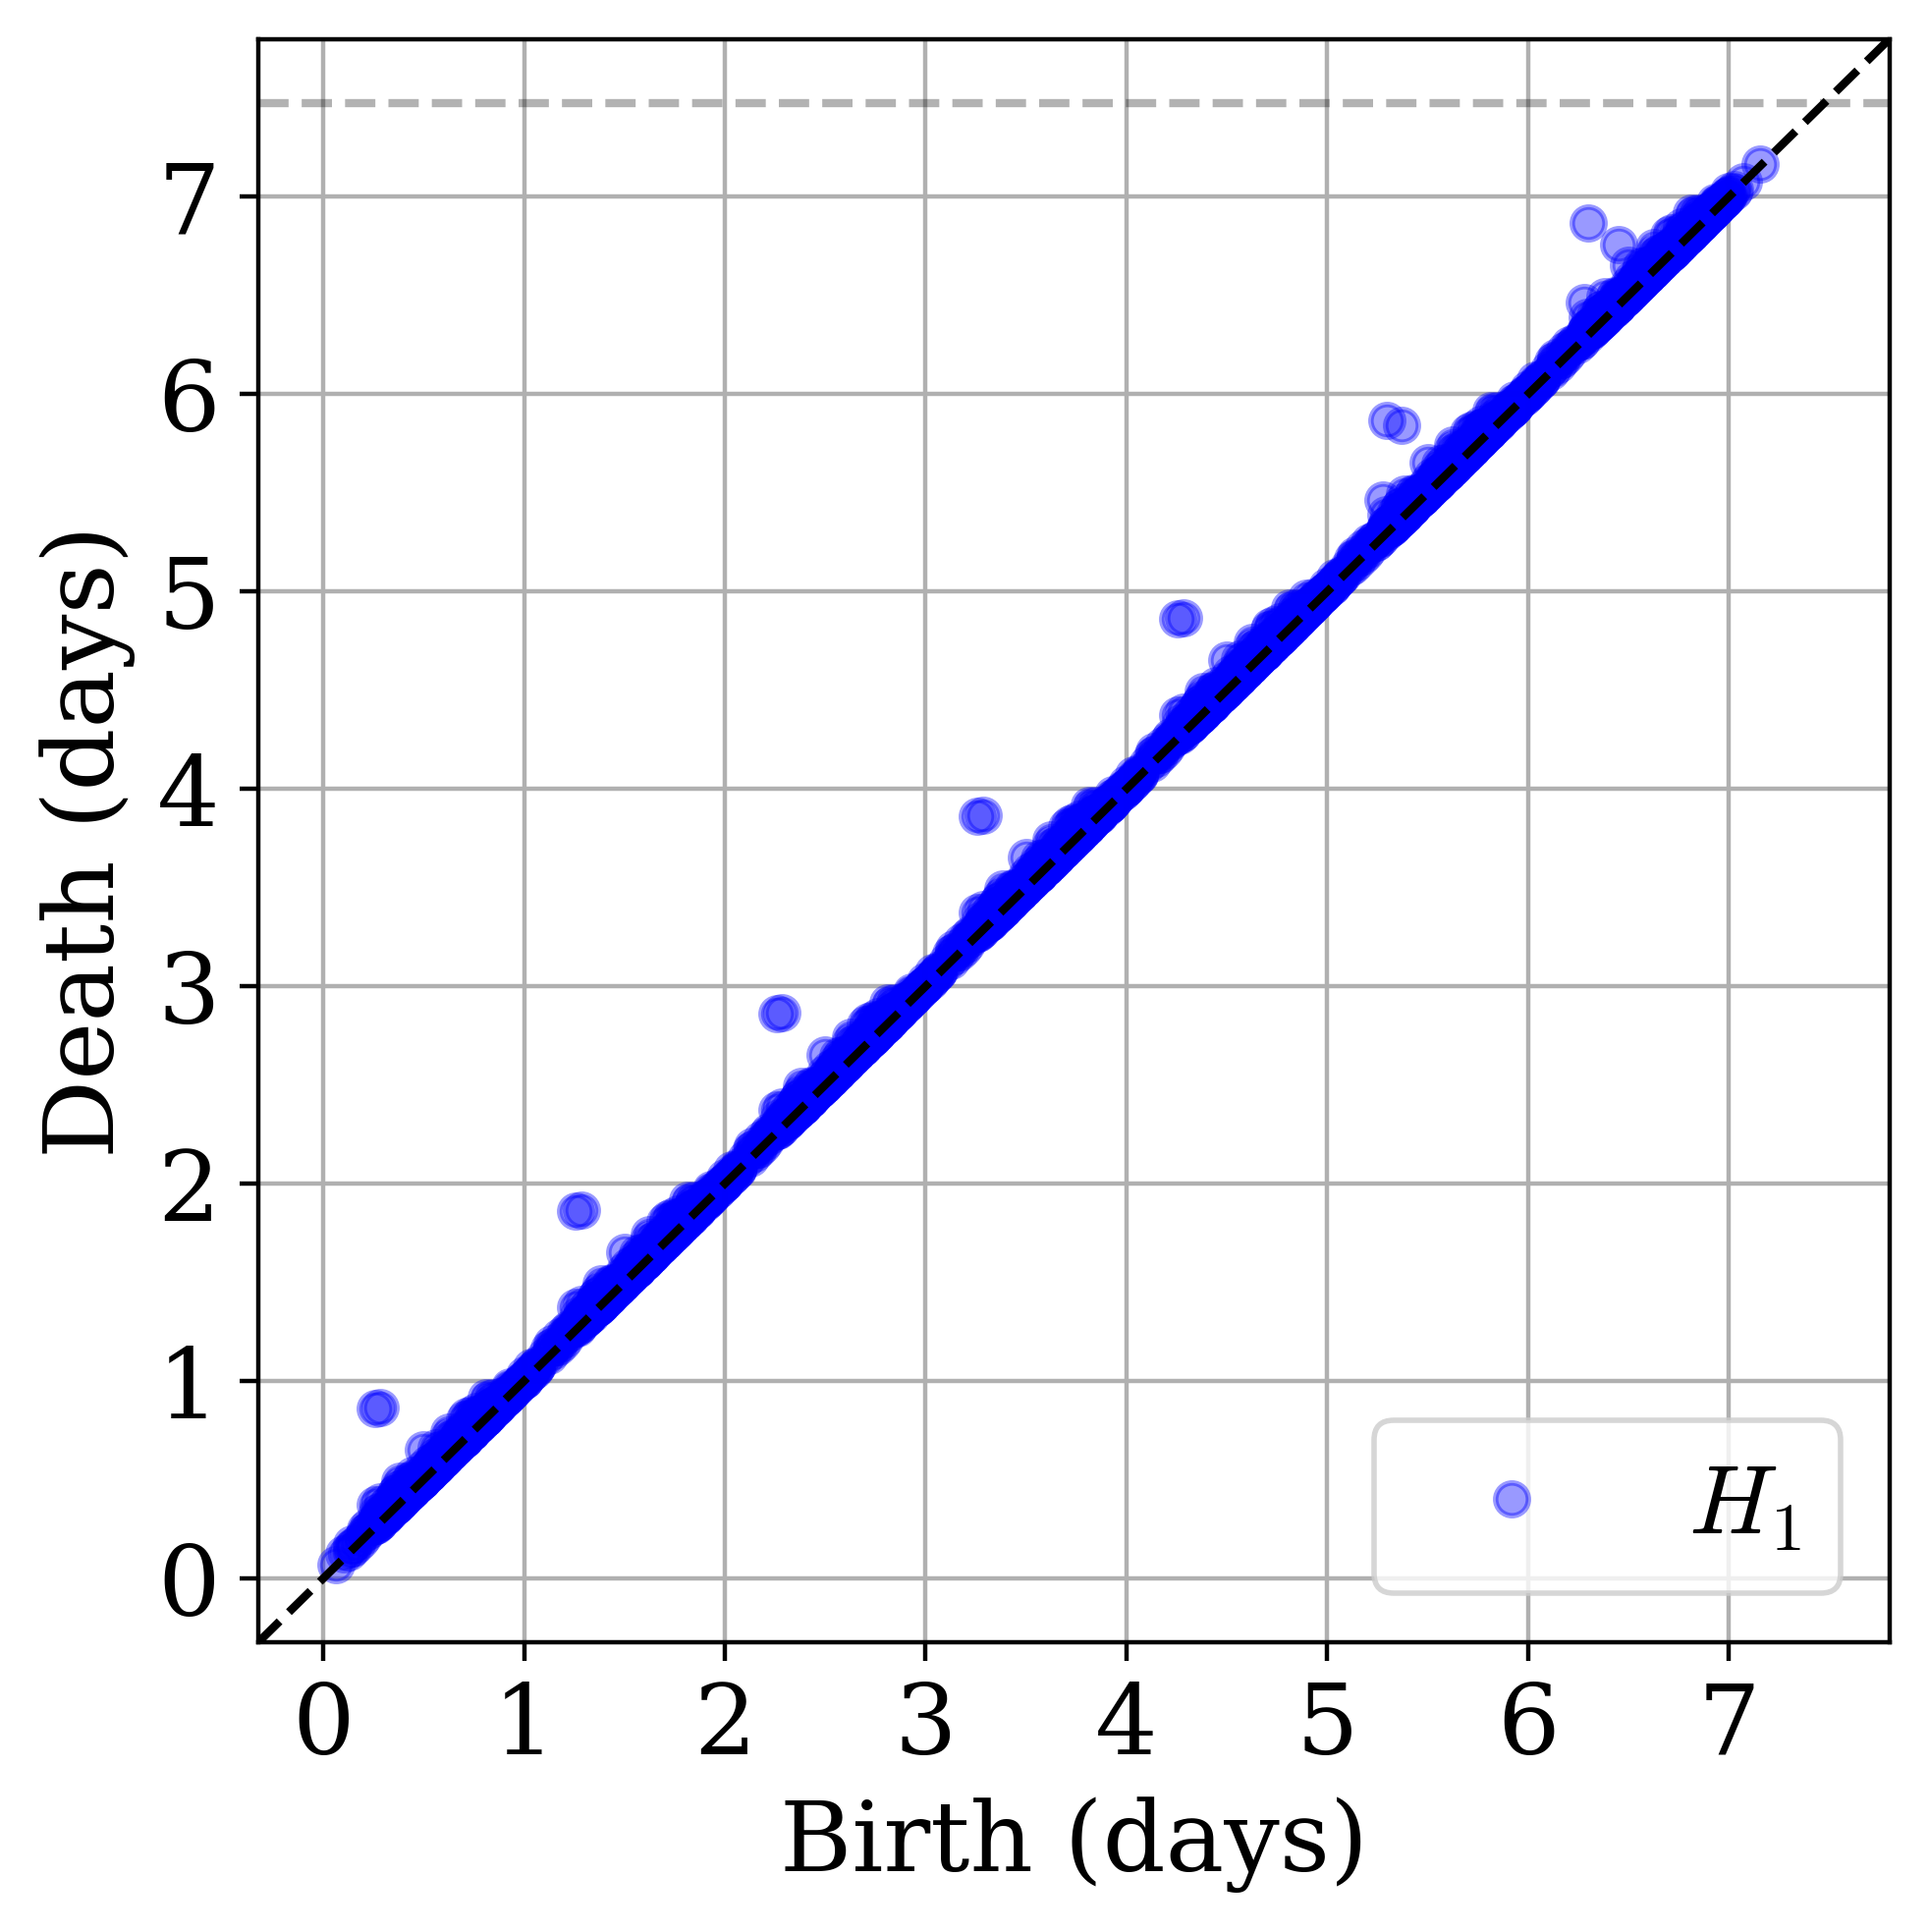
\includegraphics[width=\textwidth]{Figures/GB_coach_PD1_Rips1} \\
         (c) One-dimensional zigzag persistence.
         %
         %
     \end{minipage}

     \qquad 
     
    
\includegraphics[width=0.99\textwidth]{GB_coach_mean_centrality_components_analysis}
     (d) Connectivity and centrality analysis on temporal Great Britain coach network.
     %
     \caption{Results for the coach transportation network of Great Britain.}
     \label{fig:GB_coach_all}
\end{figure}
%
%
%
%
%


\begin{figure}
     \centering
     %
     \begin{minipage}{0.3\textwidth}
         \centering
         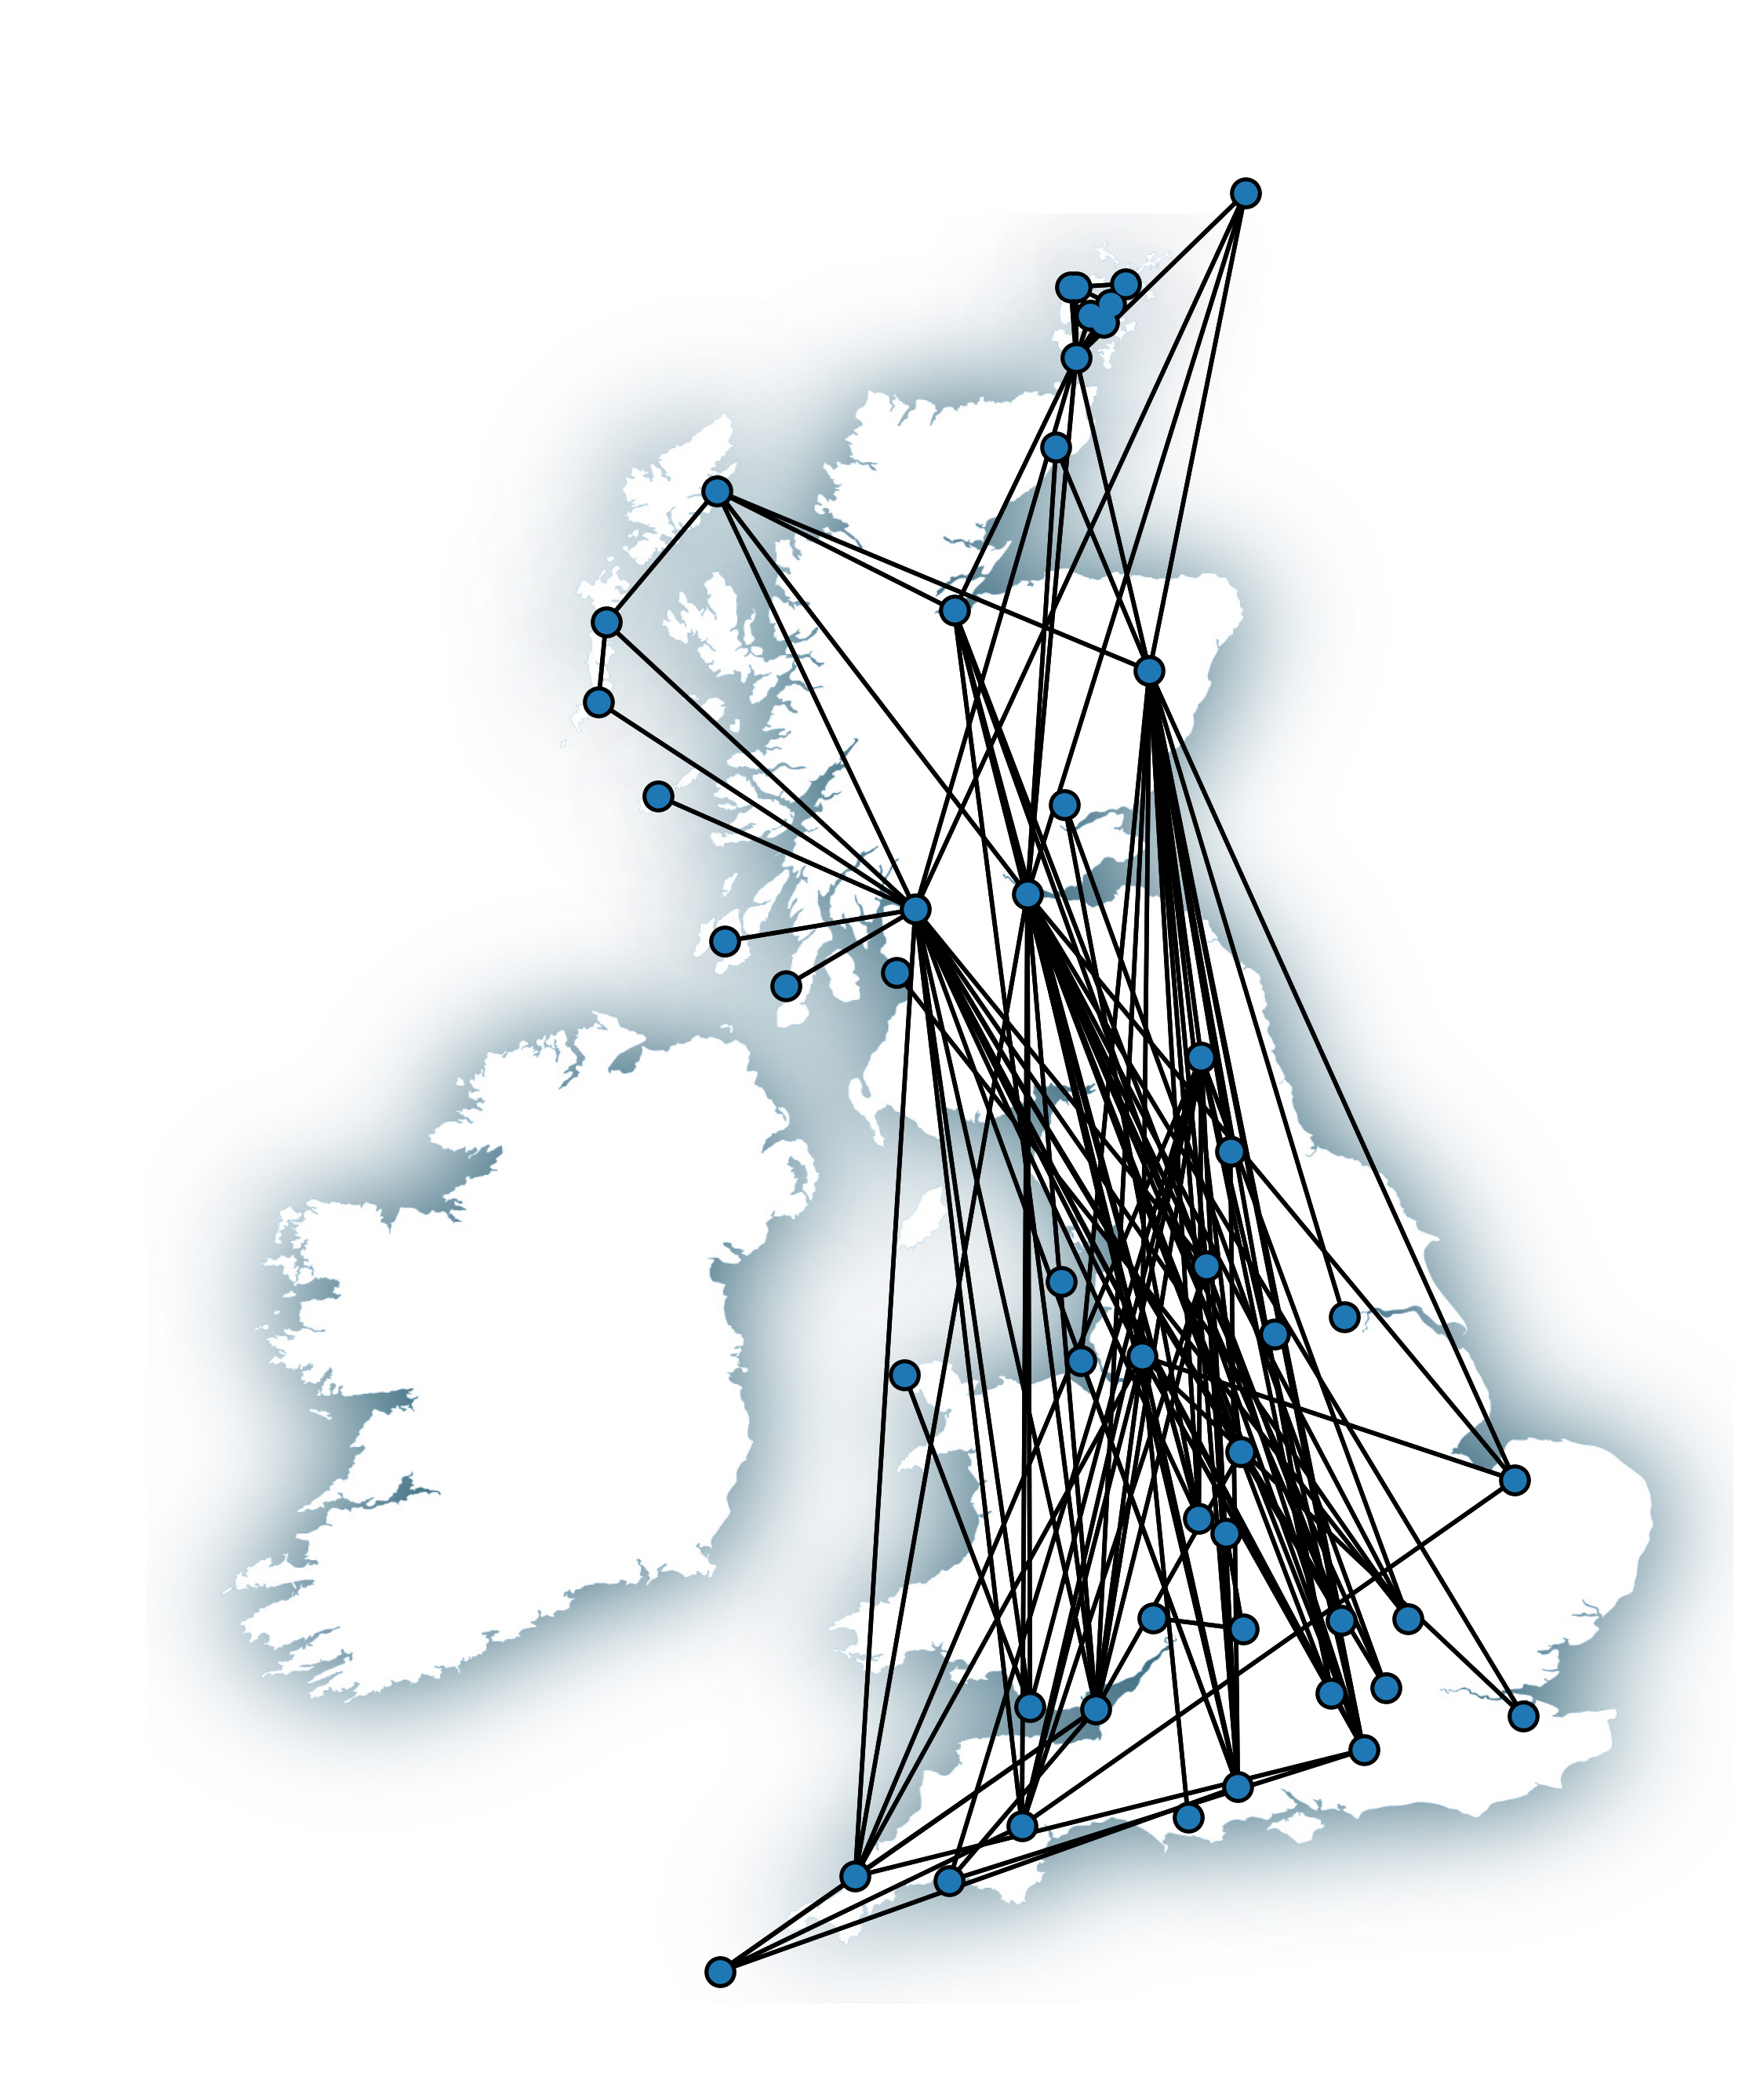
\includegraphics[width=\textwidth]{Figures/GB_air} \\
         (a) Full air Travel Network.
         %
         %
     \end{minipage}
     \hfill
     \begin{minipage}{0.3\textwidth}
         \centering
         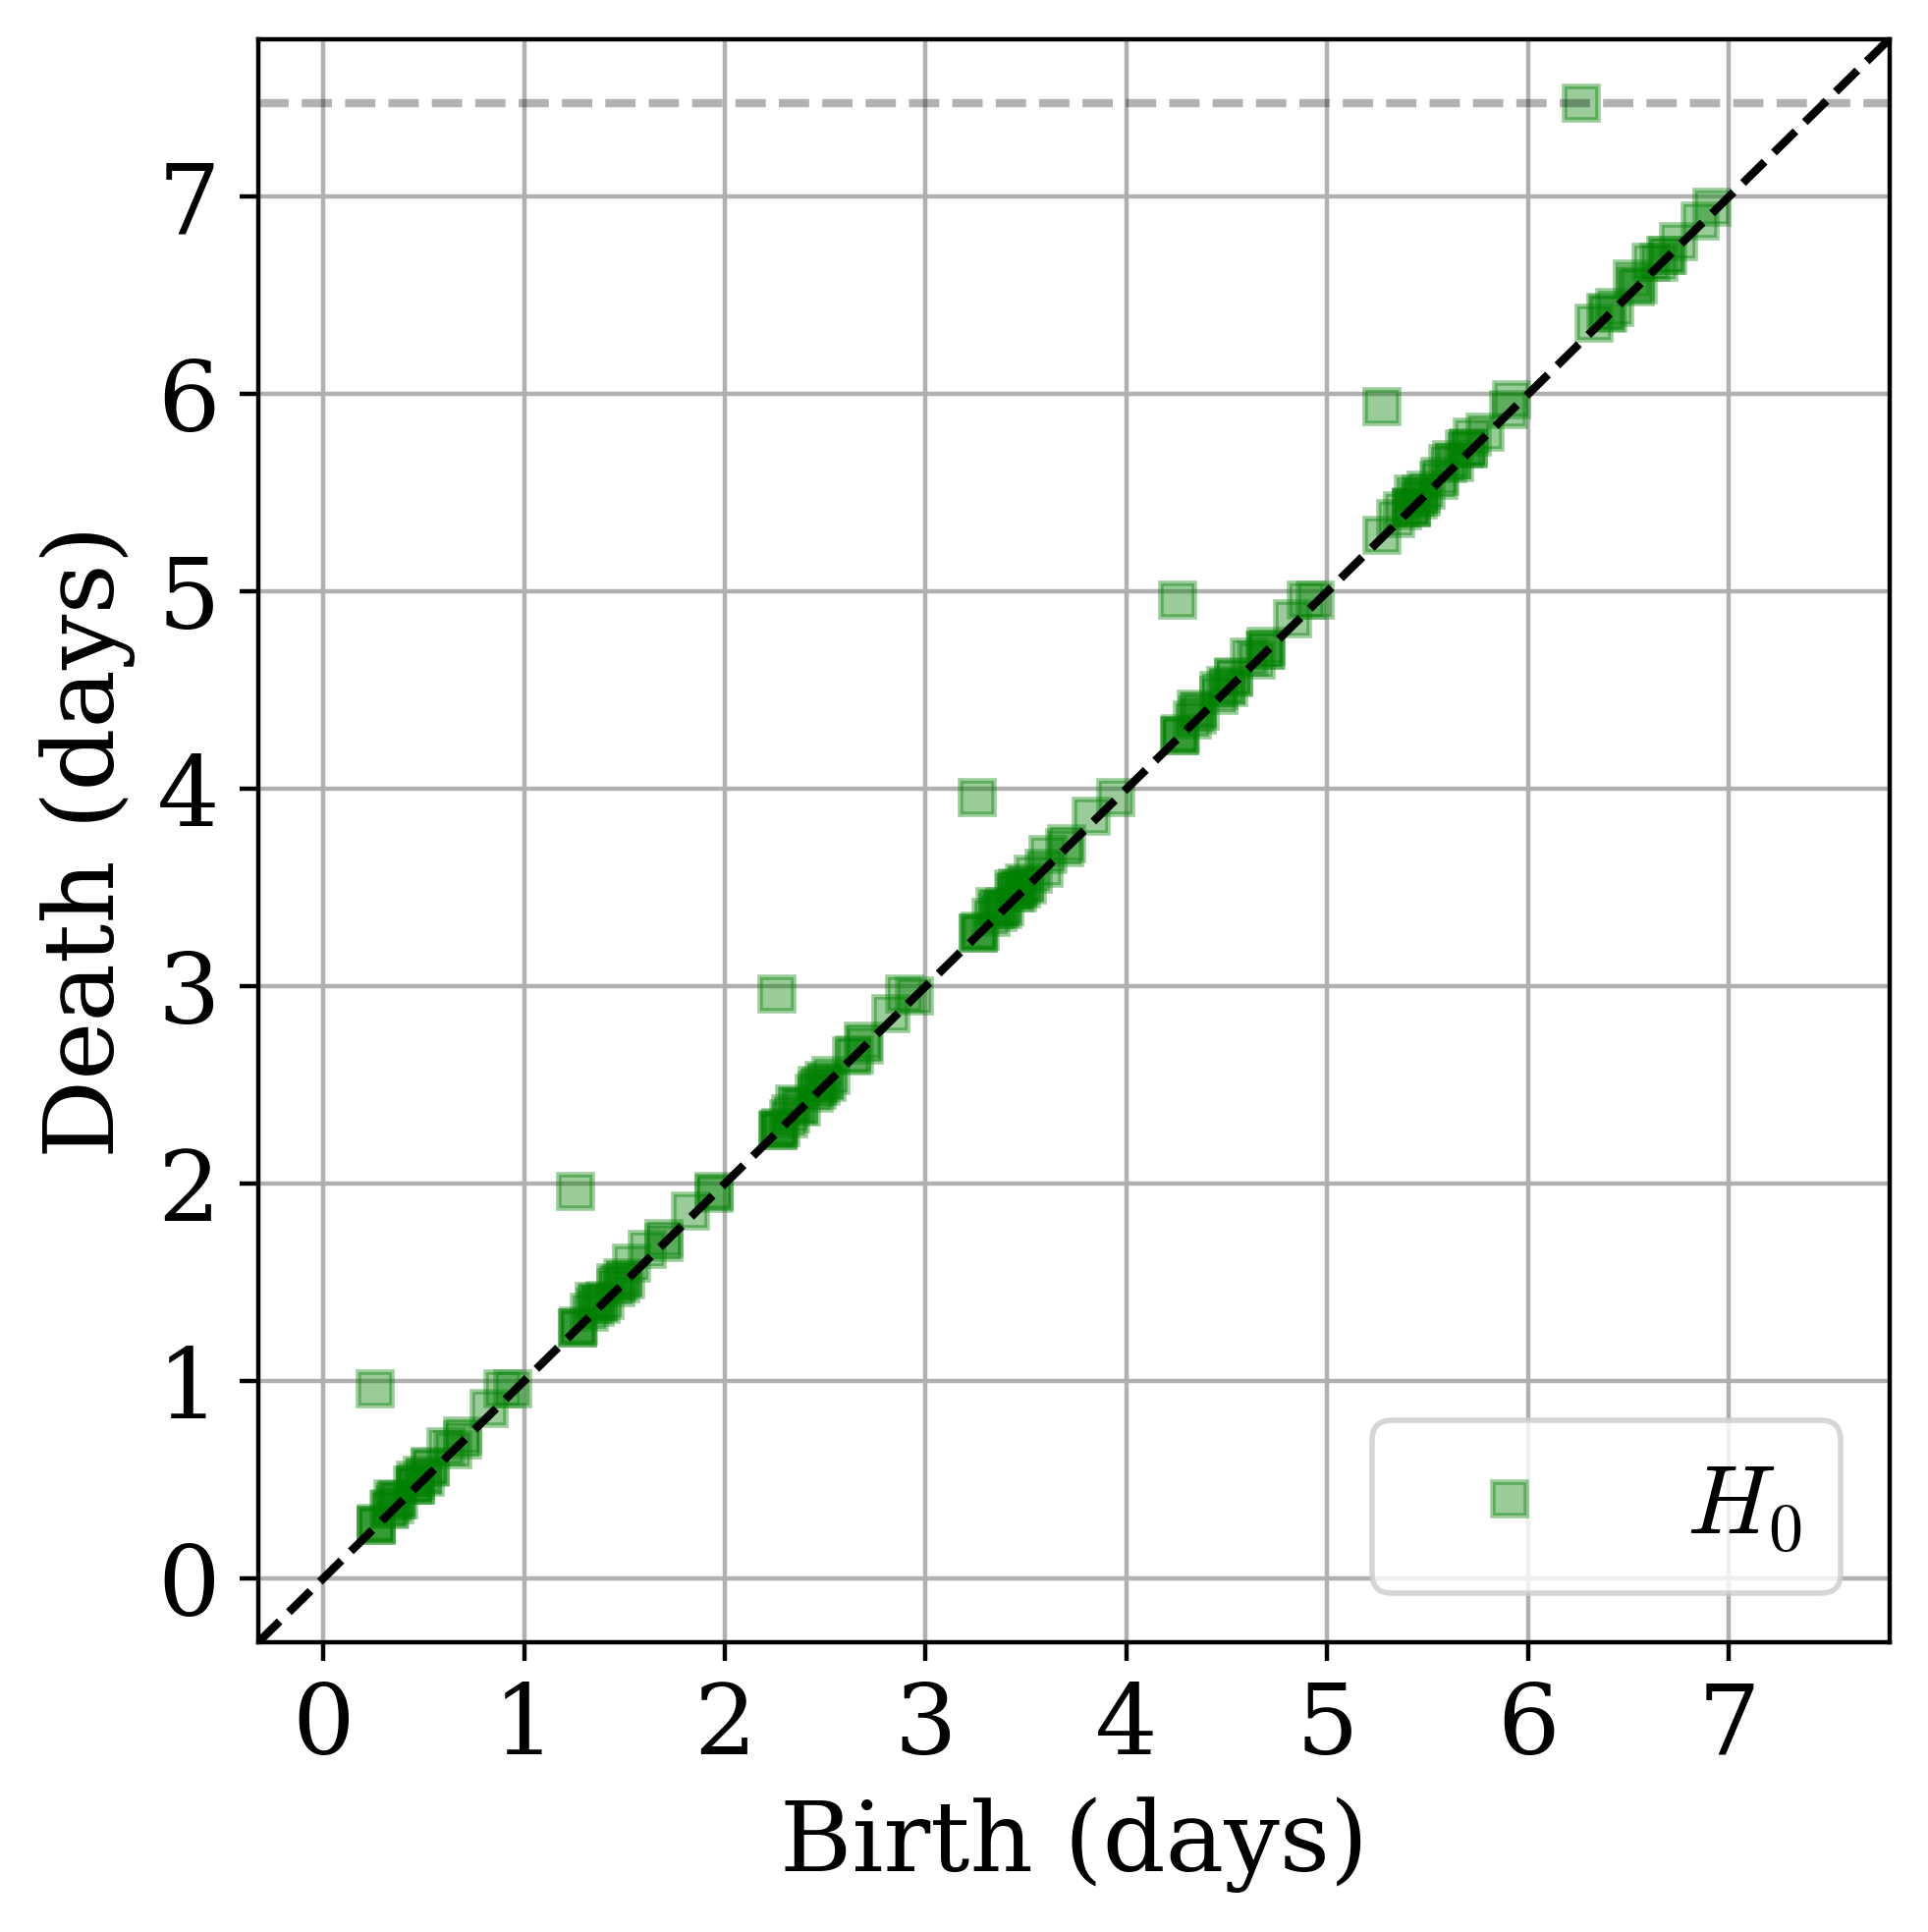
\includegraphics[width=\textwidth]{Figures/GB_air_PD0_Rips1} \\
         (b) Zero-dimensional zigzag persistence.
         %
         %
     \end{minipage}
     \hfill
     \begin{minipage}{0.3\textwidth}
         \centering
         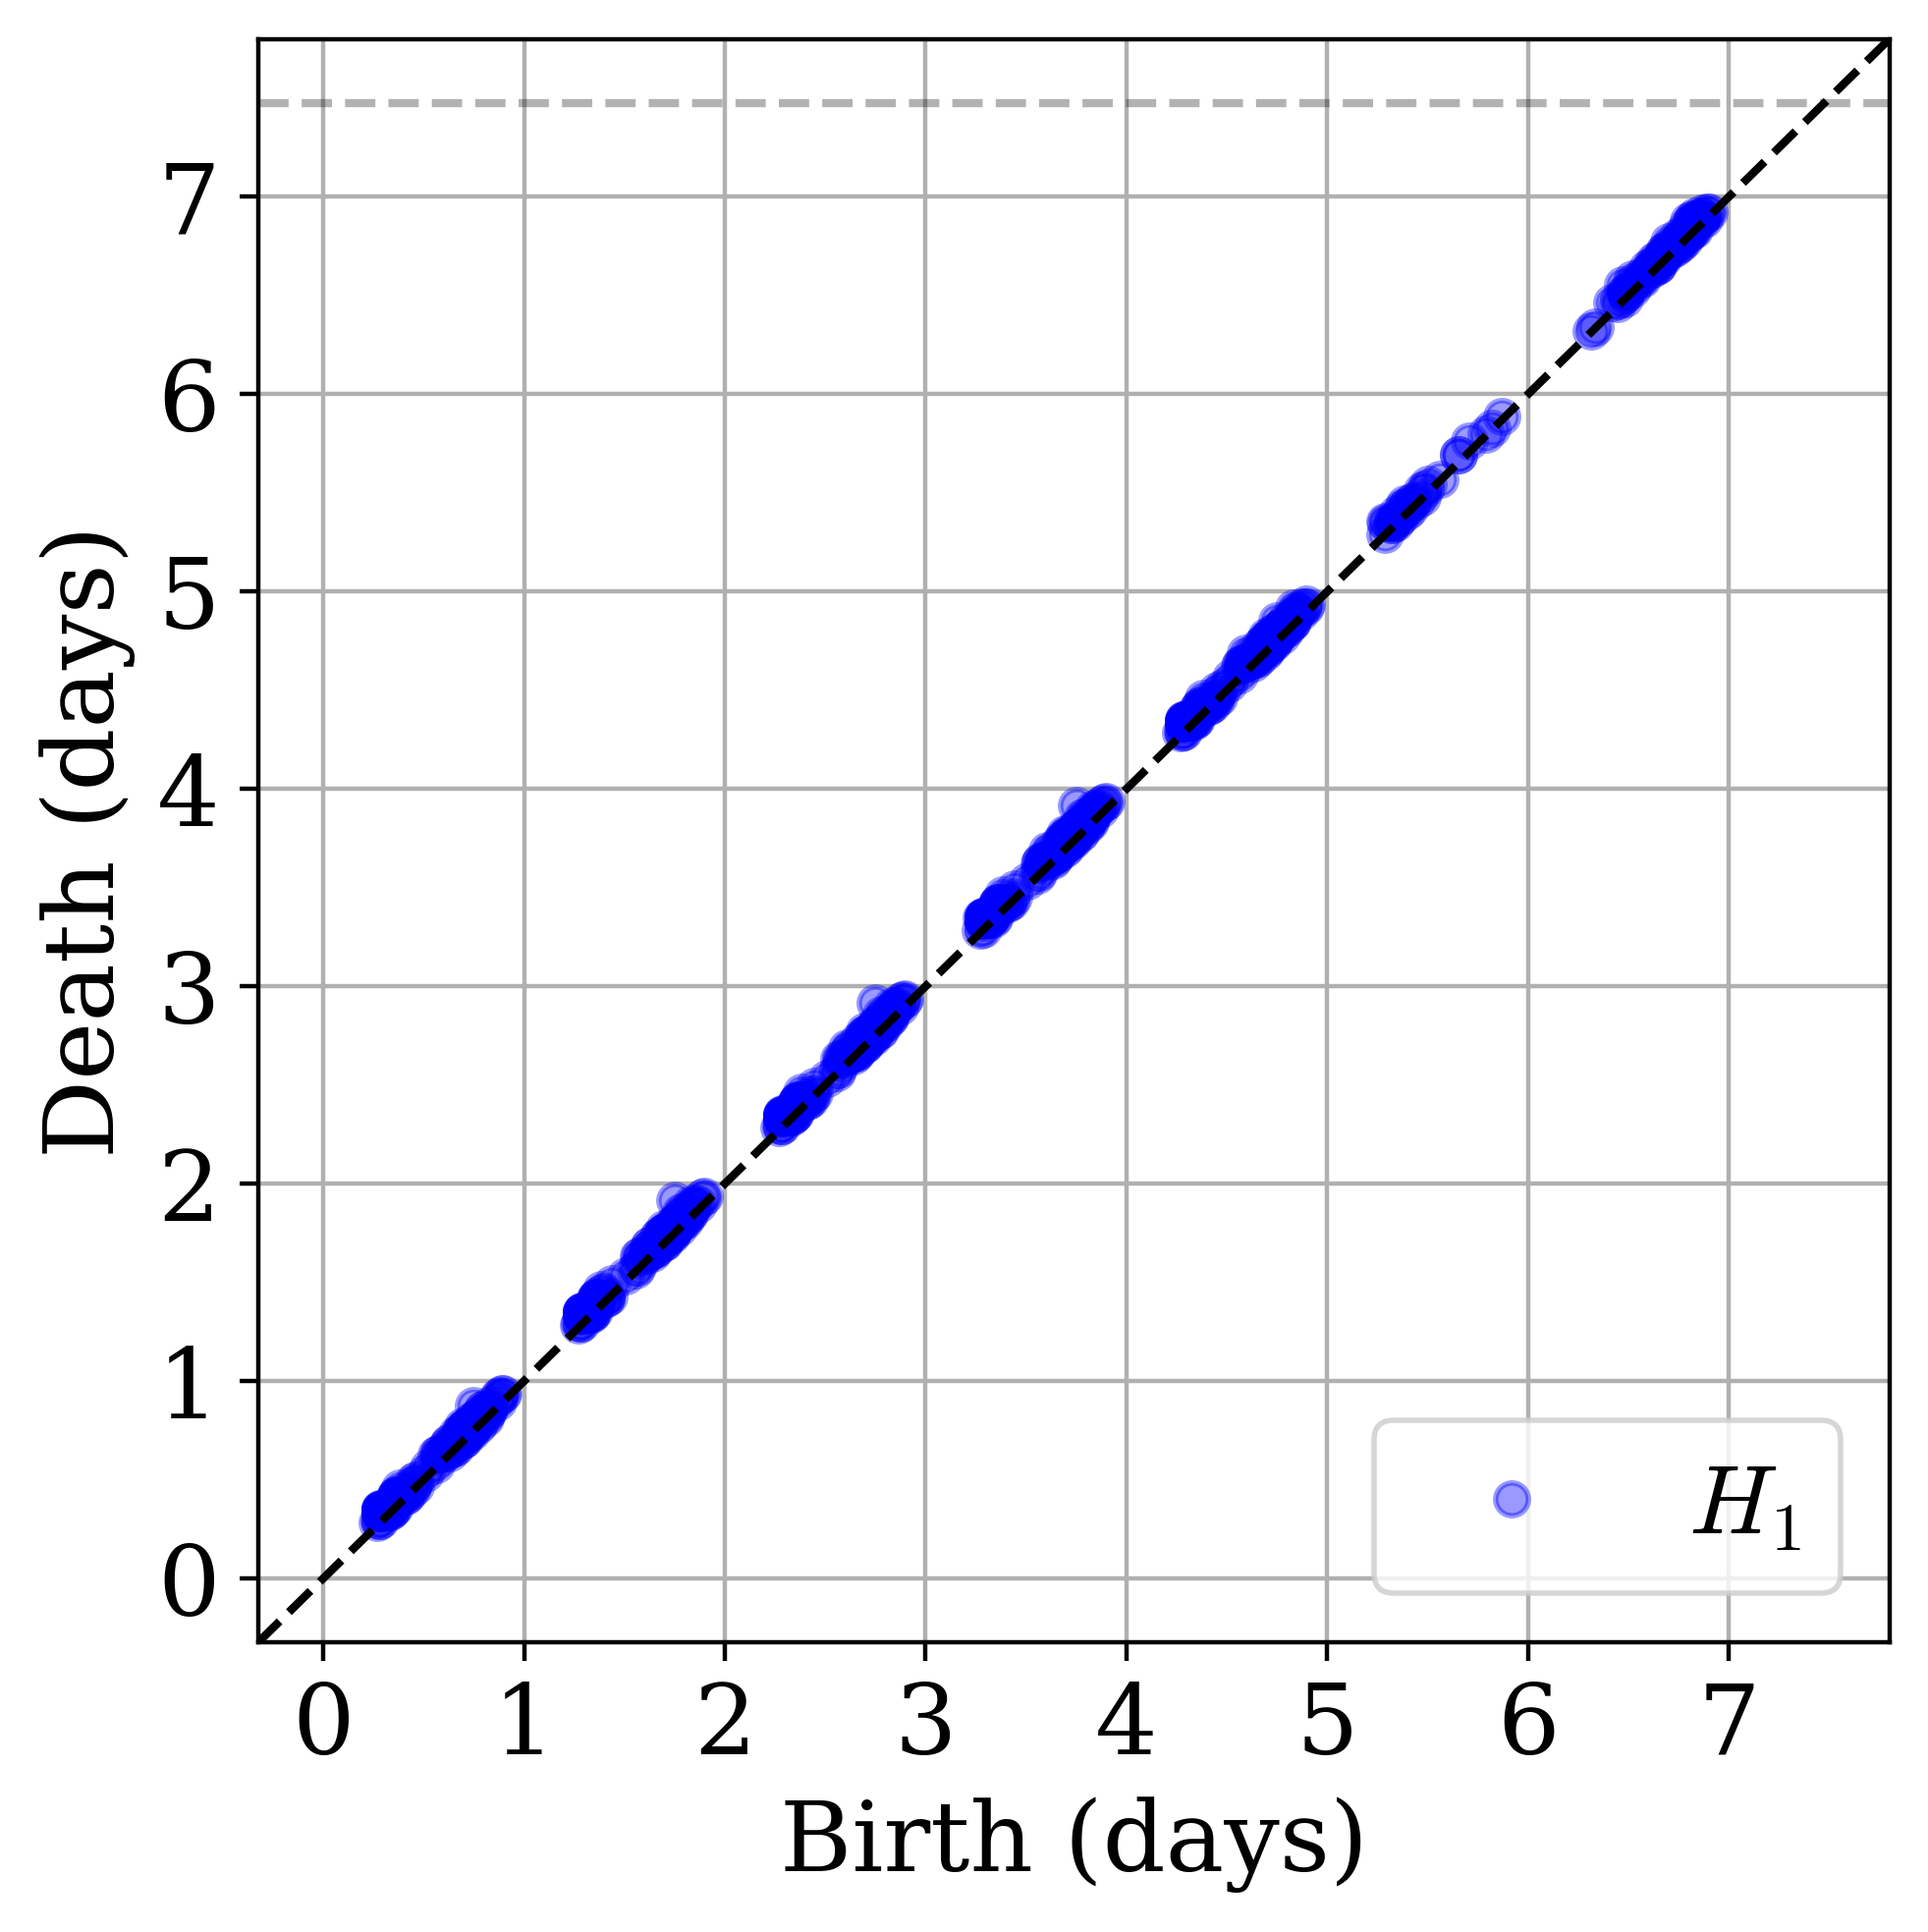
\includegraphics[width=\textwidth]{Figures/GB_air_PD1_Rips1} \\
         (c) One-dimensional zigzag persistence.
         %
         %
     \end{minipage}

     \qquad 
     
    
\includegraphics[width=0.99\textwidth]{GB_air_mean_centrality_components_analysis}
    (d)Connectivity and centrality analysis on temporal Great Britain air network.
     %
     \caption{Results for the air transportation network of Great Britain.}
     \label{fig:GB_air_all}
\end{figure}
